\documentclass[10pt,letterpaper]{article}

% ---------- Page setup ----------
\usepackage[margin=0.68in]{geometry}
\usepackage[T1]{fontenc}
\usepackage[utf8]{inputenc}
\usepackage{lmodern}
\usepackage{microtype}
\usepackage{array}
\usepackage{booktabs}
\usepackage{tabularx}
\usepackage{longtable}
\usepackage{enumitem}
\usepackage{xcolor}
\usepackage{tikz}
\usepackage[most]{tcolorbox}
\usepackage{titlesec}
\usepackage{fancyhdr}
\usepackage{lastpage}
\usepackage[hidelinks]{hyperref}
\usepackage{ragged2e}
\usepackage{multicol}
\usepackage{pifont}

% ---------- Colors ----------
\definecolor{Navy}{HTML}{17324D}
\definecolor{Blue}{HTML}{2563EB}
\definecolor{Teal}{HTML}{0F766E}
\definecolor{Green}{HTML}{15803D}
\definecolor{Amber}{HTML}{B45309}
\definecolor{Red}{HTML}{B91C1C}
\definecolor{Purple}{HTML}{6D28D9}
\definecolor{GrayText}{HTML}{475569}
\definecolor{LightBlue}{HTML}{EFF6FF}
\definecolor{LightTeal}{HTML}{ECFDF5}
\definecolor{LightAmber}{HTML}{FFFBEB}
\definecolor{LightGray}{HTML}{F8FAFC}
\definecolor{LightRed}{HTML}{FEF2F2}
\definecolor{RuleGray}{HTML}{CBD5E1}

% ---------- Global formatting ----------
\setlength{\parindent}{0pt}
\setlength{\parskip}{4pt}
\renewcommand{\arraystretch}{1.18}
\setlength{\tabcolsep}{4pt}
\setlist[itemize]{leftmargin=*, nosep, topsep=2pt}
\setlist[enumerate]{leftmargin=*, nosep, topsep=2pt}
\titleformat{\section}{\Large\bfseries\color{Navy}}{}{0em}{}[\titlerule]
\titleformat{\subsection}{\large\bfseries\color{Navy}}{}{0em}{}
\titleformat{\subsubsection}{\normalsize\bfseries\color{Navy}}{}{0em}{}
\emergencystretch=2em
\sloppy

% ---------- Header/footer ----------
\pagestyle{fancy}
\fancyhf{}
\lhead{\textcolor{GrayText}{Confluence in the Enterprise AppSec and Operations Stack}}
\rhead{\textcolor{GrayText}{Handout}}
\cfoot{\textcolor{GrayText}{Page \thepage\ of \pageref{LastPage}}}
\renewcommand{\headrulewidth}{0.4pt}
\renewcommand{\footrulewidth}{0pt}

% ---------- Column types ----------
\newcolumntype{Y}{>{\RaggedRight\arraybackslash}X}
\newcolumntype{L}[1]{>{\RaggedRight\arraybackslash}p{#1}}

% ---------- Boxes ----------
\newtcolorbox{summarybox}{
  colback=LightBlue,
  colframe=Blue,
  boxrule=0.7pt,
  arc=2mm,
  left=8pt,
  right=8pt,
  top=7pt,
  bottom=7pt
}
\newtcolorbox{principlebox}{
  colback=LightTeal,
  colframe=Teal,
  boxrule=0.7pt,
  arc=2mm,
  left=8pt,
  right=8pt,
  top=7pt,
  bottom=7pt
}
\newtcolorbox{warningbox}{
  colback=LightAmber,
  colframe=Amber,
  boxrule=0.7pt,
  arc=2mm,
  left=8pt,
  right=8pt,
  top=7pt,
  bottom=7pt
}
\newtcolorbox{riskbox}{
  colback=LightRed,
  colframe=Red,
  boxrule=0.7pt,
  arc=2mm,
  left=8pt,
  right=8pt,
  top=7pt,
  bottom=7pt
}

\newcommand{\yes}{\textcolor{Green}{\ding{51}}}
\newcommand{\no}{\textcolor{Red}{\ding{55}}}

\begin{document}

% ---------- Title ----------
{\Huge\bfseries\color{Navy} Confluence in the Enterprise AppSec and Operations Stack}\par
{\large\color{GrayText} Knowledge management, governance documentation, runbooks, and docs-as-code publishing}\par
\vspace{4pt}
{\small\color{GrayText} Prepared as a standalone architecture and operating-model reference.}\par
\vspace{10pt}

\begin{summarybox}
\textbf{Purpose.} This handout explains where Confluence fits in an Enterprise Application Security and Operations stack that includes GHAS, Trivy, OWASP ZAP, DongTai-IAST, Eramba, Taiga, GLPI, iTop, Moodle, Authentik, and SuiteCRM. Confluence is best positioned as the human-facing knowledge, runbook, and governance documentation layer. It should explain how the stack is operated, but it should not become the enforcement engine or the authoritative system of record for scanner findings, risk state, assets, training completion, or deployment decisions.
\end{summarybox}

\begin{warningbox}
\textbf{Important positioning note.} Confluence is a documentation and collaboration platform. In a strict open-source-only architecture, consider an open-source wiki or knowledge-base alternative. If the organization already uses Atlassian tooling, Confluence can provide a strong enterprise portal for AppSec standards, operational procedures, architecture records, and service documentation.
\end{warningbox}

\section{Executive Fit}

Confluence belongs in the stack as an \textbf{operating knowledge layer}. Its role is to answer the practical question: \textit{How do we operate this stack correctly?}

\begin{principlebox}
\textbf{Recommended architecture rule.} Use Git as the source of truth for versioned technical artifacts, use Confluence as the readable enterprise portal, use Moodle as the formal learning system, use Eramba as the GRC/control system, use GLPI/iTop for asset and service records, use Taiga for delivery planning, and use GHAS/Trivy/ZAP/DongTai for security execution.
\end{principlebox}

\section{Reference Placement in the Stack}

\begin{longtable}{L{1.35in} L{1.45in} L{3.65in}}
\toprule
\textbf{Layer} & \textbf{Representative Tools} & \textbf{Primary Responsibility} \\
\midrule
Identity and Access & Authentik & Centralize authentication, group mapping, access policy, and identity federation where supported. \\
Delivery Planning & Taiga & Manage epics, user stories, backlog items, sprint work, remediation tasks, and delivery coordination. \\
Security Execution & GHAS, Trivy, OWASP ZAP, DongTai-IAST & Perform source, dependency, container, dynamic, and runtime security testing. \\
Governance and Risk & Eramba & Track risks, controls, policies, exceptions, treatment plans, evidence, ownership, and compliance obligations. \\
Operations and Asset Context & GLPI, iTop & Maintain asset records, service records, configuration items, incidents, changes, and operational dependencies. \\
Training and Awareness & Moodle & Deliver formal training, quizzes, completion tracking, certificates, and role-based learning evidence. \\
Customer and Stakeholder Context & SuiteCRM & Manage account, stakeholder, customer, and relationship workflows where appropriate. \\
\textbf{Knowledge and Runbooks} & \textbf{Confluence} & \textbf{Publish the operating model, standards, procedures, runbooks, service catalog, architecture decisions, and cross-tool guidance.} \\
\bottomrule
\end{longtable}

\section{Architecture View}

\begin{center}
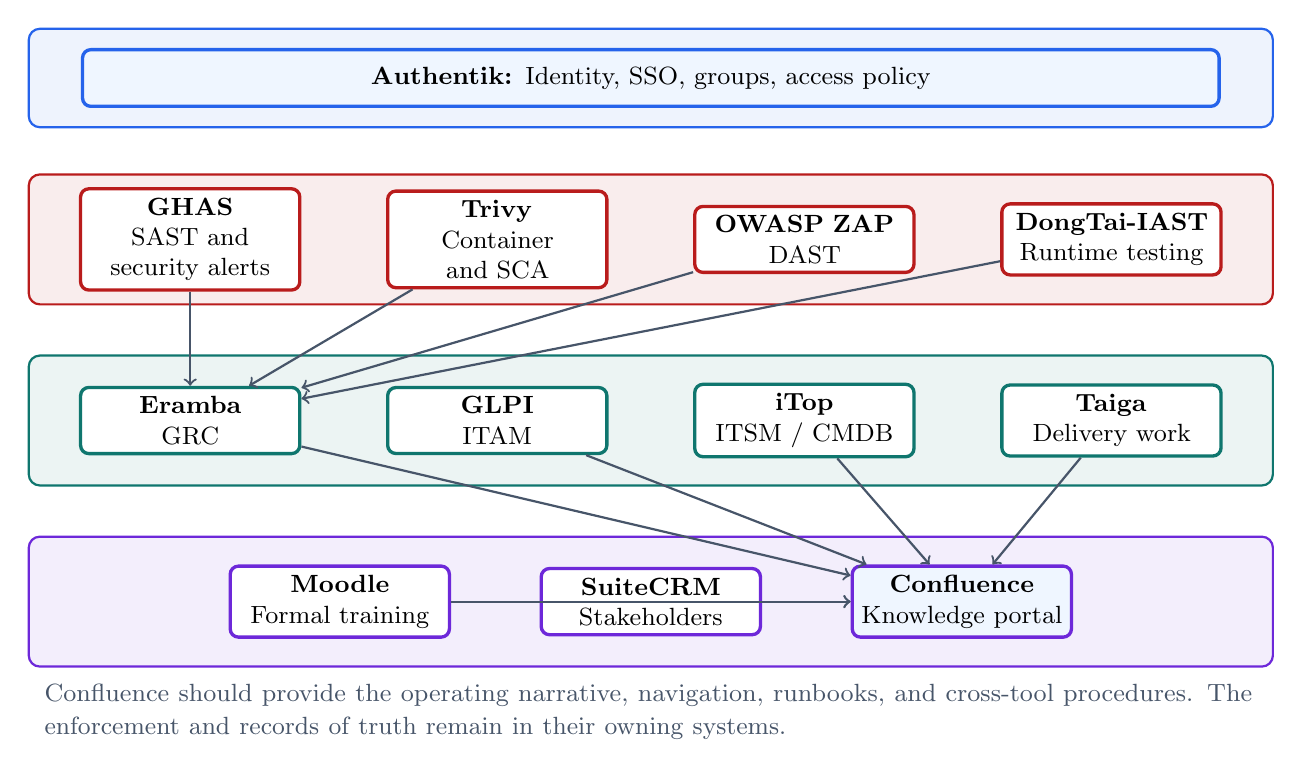
\begin{tikzpicture}[
  node distance=0.55cm,
  box/.style={rectangle, rounded corners=3pt, draw=RuleGray, very thick, align=center, minimum height=0.62cm, text width=2.55cm, fill=white, font=\small},
  widebox/.style={rectangle, rounded corners=3pt, draw=RuleGray, very thick, align=center, minimum height=0.72cm, text width=14.2cm, fill=white, font=\small},
  layer/.style={rectangle, rounded corners=4pt, draw=#1, thick, fill=#1!8, inner sep=7pt},
  arrow/.style={->, thick, draw=GrayText}
]

\node[layer=Blue, minimum width=15.8cm, minimum height=1.25cm] at (0,0) {};
\node[widebox, draw=Blue, fill=LightBlue] (identity) at (0,0) {\textbf{Authentik:} Identity, SSO, groups, access policy};

\node[layer=Red, minimum width=15.8cm, minimum height=1.65cm] at (0,-2.05) {};
\node[box, draw=Red] (ghas) at (-5.85,-2.05) {\textbf{GHAS}\\SAST and security alerts};
\node[box, draw=Red] (trivy) at (-1.95,-2.05) {\textbf{Trivy}\\Container and SCA};
\node[box, draw=Red] (zap) at (1.95,-2.05) {\textbf{OWASP ZAP}\\DAST};
\node[box, draw=Red] (dongtai) at (5.85,-2.05) {\textbf{DongTai-IAST}\\Runtime testing};

\node[layer=Teal, minimum width=15.8cm, minimum height=1.65cm] at (0,-4.35) {};
\node[box, draw=Teal] (eramba) at (-5.85,-4.35) {\textbf{Eramba}\\GRC};
\node[box, draw=Teal] (glpi) at (-1.95,-4.35) {\textbf{GLPI}\\ITAM};
\node[box, draw=Teal] (itop) at (1.95,-4.35) {\textbf{iTop}\\ITSM / CMDB};
\node[box, draw=Teal] (taiga) at (5.85,-4.35) {\textbf{Taiga}\\Delivery work};

\node[layer=Purple, minimum width=15.8cm, minimum height=1.65cm] at (0,-6.65) {};
\node[box, draw=Purple] (moodle) at (-3.95,-6.65) {\textbf{Moodle}\\Formal training};
\node[box, draw=Purple] (suitecrm) at (0,-6.65) {\textbf{SuiteCRM}\\Stakeholders};
\node[box, draw=Purple, fill=LightBlue] (confluence) at (3.95,-6.65) {\textbf{Confluence}\\Knowledge portal};

\draw[arrow] (ghas) -- (eramba);
\draw[arrow] (trivy) -- (eramba);
\draw[arrow] (zap) -- (eramba);
\draw[arrow] (dongtai) -- (eramba);
\draw[arrow] (eramba) -- (confluence);
\draw[arrow] (glpi) -- (confluence);
\draw[arrow] (itop) -- (confluence);
\draw[arrow] (taiga) -- (confluence);
\draw[arrow] (moodle) -- (confluence);
\draw[arrow] (suitecrm) -- (confluence);

\node[align=left, text width=15.4cm, color=GrayText] at (0,-8.05) {\small Confluence should provide the operating narrative, navigation, runbooks, and cross-tool procedures. The enforcement and records of truth remain in their owning systems.};
\end{tikzpicture}
\end{center}

\section{What Confluence Should Own}

\begin{tabularx}{\textwidth}{L{1.85in} Y}
\toprule
\textbf{Knowledge Area} & \textbf{Recommended Confluence Content} \\
\midrule
AppSec Operating Model & AppSec service catalog, intake model, review workflow, triage model, severity expectations, escalation model, and roles/responsibilities. \\
GHAS Operations & Code scanning onboarding, secret scanning response, alert triage procedures, dismissal criteria, delegated approval process, evidence requirements, and repository onboarding checklist. \\
CI/CD and Release Governance & Pipeline gate descriptions, deployment approval criteria, build/release runbooks, rollback procedures, promotion flow, and release readiness guidance. \\
Security Tooling Guides & ZAP scan procedure, Trivy container scan handling, DongTai-IAST QA usage, scanner ownership, false-positive process, and remediation playbooks. \\
GRC Procedures & Policy lifecycle, control evidence procedures, exception handling, risk acceptance workflow, audit support process, and Eramba operating instructions. \\
Operations Runbooks & Incident triage, change handling, service ownership lookup, asset ownership lookup, CMDB usage guidance, and GLPI/iTop work instructions. \\
Architecture Knowledge & Architecture decision records, system context diagrams, integration maps, security architecture views, capability maps, and platform roadmaps. \\
Onboarding and Enablement & New engineer onboarding, AppSec onboarding, tool access instructions, team-specific starter guides, and links to Moodle courses. \\
\bottomrule
\end{tabularx}

\section{What Confluence Should Not Own}

\begin{riskbox}
\textbf{Avoid the wiki-as-database antipattern.} Confluence pages are excellent for explanation and navigation, but they become brittle when used as the authoritative source for fast-changing operational records.
\end{riskbox}

\begin{tabularx}{\textwidth}{L{2.15in} L{2.2in} Y}
\toprule
\textbf{Do Not Make Confluence Authoritative For} & \textbf{Better System of Record} & \textbf{Reason} \\
\midrule
Security findings and alert state & GHAS, Trivy, OWASP ZAP, DongTai-IAST & Findings change frequently and need scanner-native status, severity, evidence, and lifecycle state. \\
Control status and risk treatment & Eramba & GRC requires structured control mapping, exception tracking, ownership, evidence, and reporting. \\
Asset inventory and ownership & GLPI & Asset records require lifecycle, inventory, ownership, software, and hardware state. \\
Service records and configuration items & iTop & CMDB/service records require relationships, incidents, changes, and dependency mapping. \\
Training completion and assessments & Moodle & Formal learning systems track enrollments, completions, quizzes, certificates, and evidence. \\
Project backlog and sprint delivery & Taiga & Work management needs status, assignees, priorities, estimates, and sprint flow. \\
Access decisions and identity policy & Authentik & Access control needs identity lifecycle, groups, federation, and authentication policy. \\
\bottomrule
\end{tabularx}

\section{Tool-by-Tool Integration Map}

\begin{longtable}{L{1.2in} L{2.1in} L{3.45in}}
\toprule
\textbf{Tool} & \textbf{Confluence Relationship} & \textbf{Recommended Page Types} \\
\midrule
GHAS & Document security scanning standards and developer-facing response procedures. & Repository onboarding guide, CodeQL rules guidance, alert triage matrix, dismissal evidence checklist, delegated approval standard. \\
Trivy & Explain container and dependency scan interpretation. & Image scanning runbook, severity threshold policy, remediation workflow, exception request procedure. \\
OWASP ZAP & Standardize DAST execution and result handling. & Scan setup procedure, target onboarding guide, false-positive handling, authenticated scan checklist. \\
DongTai-IAST & Explain QA-stage runtime testing expectations. & IAST test procedure, environment prerequisites, finding interpretation guide, evidence collection checklist. \\
Eramba & Link policies, controls, risks, exceptions, and audit support procedures. & GRC operating model, control owner guide, risk acceptance procedure, evidence submission checklist. \\
Taiga & Provide delivery standards and links to relevant epics/stories. & Backlog taxonomy, user story standard, remediation delivery workflow, sprint operating model. \\
GLPI & Explain asset ownership and inventory maintenance. & Asset intake guide, ownership update procedure, software inventory standard, asset lifecycle checklist. \\
iTop & Explain service management and CMDB usage. & CI/service mapping guide, incident/change runbook, service catalog page template, dependency mapping instructions. \\
Moodle & Link lightweight references to formal training. & Course companion page, role-based training path, procedure summary, compliance training index. \\
Authentik & Document access model and SSO expectations. & Access request guide, group mapping reference, application onboarding checklist, privileged access procedure. \\
SuiteCRM & Document stakeholder and customer workflow guidance. & Stakeholder engagement procedure, account-support handoff, customer communication standard. \\
\bottomrule
\end{longtable}

\section{Docs-as-Code Publishing Pattern}

The cleanest pattern is to keep controlled technical artifacts in Git and publish curated versions into Confluence for enterprise consumption.

\begin{center}
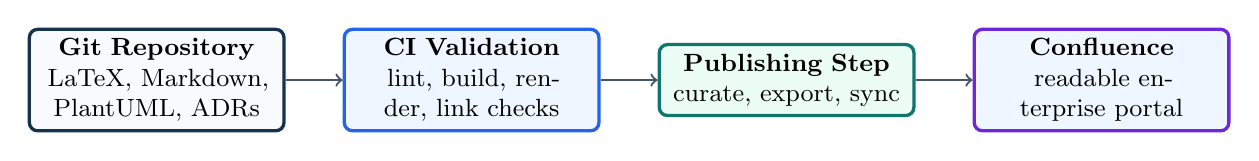
\begin{tikzpicture}[
  node distance=0.8cm,
  box/.style={rectangle, rounded corners=3pt, draw=RuleGray, very thick, align=center, minimum height=0.74cm, text width=3.0cm, fill=white, font=\small},
  arrow/.style={->, thick, draw=GrayText}
]
\node[box, draw=Navy, fill=LightGray] (git) at (0,0) {\textbf{Git Repository}\\LaTeX, Markdown, PlantUML, ADRs};
\node[box, draw=Blue, fill=LightBlue] (ci) at (4.0,0) {\textbf{CI Validation}\\lint, build, render, link checks};
\node[box, draw=Teal, fill=LightTeal] (publish) at (8.0,0) {\textbf{Publishing Step}\\curate, export, sync};
\node[box, draw=Purple, fill=LightBlue] (conf) at (12.0,0) {\textbf{Confluence}\\readable enterprise portal};
\draw[arrow] (git) -- (ci);
\draw[arrow] (ci) -- (publish);
\draw[arrow] (publish) -- (conf);
\end{tikzpicture}
\end{center}

\subsection{Recommended Source-of-Truth Model}

\begin{tabularx}{\textwidth}{L{1.85in} L{2.2in} Y}
\toprule
\textbf{Artifact Type} & \textbf{Best Source of Truth} & \textbf{Confluence Role} \\
\midrule
Policies and standards & Git plus GRC approval record & Publish approved readable versions and link to control mappings. \\
Architecture diagrams & Git, PlantUML, draw.io source, or architecture repository & Display diagrams, explain context, and link to source. \\
Runbooks and procedures & Git for controlled runbooks; Confluence for operational presentation & Host human-readable steps, prerequisites, success criteria, and escalation paths. \\
Training modules & Moodle & Provide companion pages and link to required courses. \\
Control evidence records & Eramba & Explain how to submit evidence and link to authoritative evidence records. \\
Asset/service ownership & GLPI/iTop & Explain lookup procedures and link to records. \\
\bottomrule
\end{tabularx}

\section{Recommended Confluence Space Architecture}

\begin{longtable}{L{1.85in} L{4.9in}}
\toprule
\textbf{Space} & \textbf{Purpose} \\
\midrule
AppSec Program & AppSec operating model, secure SDLC, GHAS triage, vulnerability management, service catalog, standards, exception process. \\
DevSecOps Platform & CI/CD architecture, deployment gates, pipeline standards, GitHub Actions guidance, release runbooks, rollback procedures. \\
Security Tooling & GHAS, Trivy, OWASP ZAP, DongTai-IAST, Authentik, and other tool-specific operating guides. \\
GRC and Compliance & Policies, control mappings, evidence procedures, risk acceptance, audit support, Eramba process documentation. \\
IT Operations & iTop and GLPI procedures, service ownership, asset ownership, incident/change/problem workflows, and CMDB guidance. \\
Architecture Repository & Architecture decision records, capability maps, system context diagrams, integration diagrams, platform roadmaps. \\
Service Catalog & AppSec services, intake criteria, SLAs, support channels, service owners, request paths. \\
Training Companion & Lightweight references that map to formal Moodle courses and role-based learning paths. \\
\bottomrule
\end{longtable}

\section{Core Page Templates}

\subsection{Runbook Template}

\begin{tabularx}{\textwidth}{L{1.6in} Y}
\toprule
\textbf{Section} & \textbf{Required Content} \\
\midrule
Purpose & State the operational task and the outcome the user should achieve. \\
Scope & Define systems, teams, environments, and exclusions. \\
Prerequisites & Required access, tools, permissions, inputs, tickets, and approvals. \\
Procedure & Numbered steps with decision points, expected outputs, and handoffs. \\
Success Criteria & Observable conditions that prove completion. \\
Escalation & Owner, support group, Slack/Teams channel, service desk path, or on-call path. \\
Evidence & Screenshots, logs, ticket links, scan reports, or GRC evidence records required. \\
Revision Control & Owner, approver, review cadence, last reviewed date, and related source artifact. \\
\bottomrule
\end{tabularx}

\subsection{Architecture Decision Record Template}

\begin{tabularx}{\textwidth}{L{1.6in} Y}
\toprule
\textbf{Section} & \textbf{Required Content} \\
\midrule
Status & Proposed, accepted, superseded, deprecated, or rejected. \\
Context & Constraints, forces, requirements, and stakeholder concerns. \\
Decision & The selected approach in concise terms. \\
Consequences & Operational, security, cost, maintainability, and compliance effects. \\
Alternatives & Other options considered and why they were not chosen. \\
References & Links to diagrams, tickets, standards, risk records, and implementation work. \\
\bottomrule
\end{tabularx}

\section{Governance Controls for Confluence}

\begin{enumerate}
  \item \textbf{Define ownership.} Every critical page should have a named owner and accountable team.
  \item \textbf{Define review cadence.} AppSec standards, runbooks, and service catalog pages should have a recurring review interval.
  \item \textbf{Separate draft and approved content.} Use status labels such as draft, under review, approved, deprecated, and superseded.
  \item \textbf{Restrict sensitive spaces.} Privileged runbooks, incident procedures, architecture details, and security procedures should use controlled access.
  \item \textbf{Avoid stale operational data.} Link to GHAS, Eramba, GLPI, iTop, Taiga, and Moodle records rather than manually copying volatile state.
  \item \textbf{Use standard page templates.} Standard templates improve readability, auditability, onboarding speed, and operational consistency.
  \item \textbf{Maintain source links.} Pages generated from Git should point back to the authoritative source repository and commit or release tag where practical.
\end{enumerate}

\section{Decision Guidance}

\begin{tabularx}{\textwidth}{L{1.75in} Y}
\toprule
\textbf{Use This System} & \textbf{When the Question Is} \\
\midrule
Git & What is the controlled source version of this policy, diagram, script, standard, or technical artifact? \\
Confluence & How do I understand, operate, request, or follow this process? \\
Moodle & Who has completed the required training, course, quiz, or certification activity? \\
Eramba & What control, risk, exception, evidence, or compliance obligation applies? \\
GLPI & What asset exists, who owns it, and what is its lifecycle state? \\
iTop & What service or CI is affected, and how does it relate to incidents, changes, and dependencies? \\
Taiga & What work is planned, assigned, prioritized, estimated, or in progress? \\
GHAS/Trivy/ZAP/DongTai & What security finding exists, what is its severity, and what is its scanner-native state? \\
Authentik & Who can access the system, through what identity group, and under what authentication policy? \\
\bottomrule
\end{tabularx}

\section{Implementation Roadmap}

\begin{longtable}{L{1.1in} L{2.1in} L{3.55in}}
\toprule
\textbf{Phase} & \textbf{Goal} & \textbf{Key Deliverables} \\
\midrule
1 & Establish Confluence governance & Space structure, ownership model, access model, page templates, labeling standard, review cadence. \\
2 & Publish core operating model & AppSec service catalog, DevSecOps platform overview, GHAS triage guide, vulnerability management procedure. \\
3 & Integrate with tool ecosystem & Links to GHAS, Eramba, Taiga, GLPI, iTop, Moodle, and identity/access guidance. \\
4 & Adopt docs-as-code workflow & Git-based source artifacts, validation pipeline, publishing workflow, source links, review process. \\
5 & Operationalize maintenance & Quarterly review cycle, stale-page reporting, owner accountability, deprecation process, audit readiness checks. \\
\bottomrule
\end{longtable}

\section{Bottom Line}

Confluence should be treated as the \textbf{readable enterprise portal} for the stack. It ties together security tooling, governance systems, operations systems, training, identity, and delivery planning by documenting how people should use them.

\begin{summarybox}
\textbf{Recommended final model.}
\begin{center}
\textbf{Git} = source of truth \quad
\textbf{Confluence} = readable enterprise portal \quad
\textbf{Moodle} = formal training \quad
\textbf{Eramba} = GRC/control system \quad
\textbf{GLPI/iTop} = asset and service records \quad
\textbf{Taiga} = delivery planning \quad
\textbf{GHAS/Trivy/ZAP/DongTai} = security execution
\end{center}
\end{summarybox}

\end{document}
